%%
%% UnBTeX: A class for bachelor, master, and doctoral thesis at the
%% University of Brasilia (UnB), Brazil
%% Version 1.1.3 2022/09/04
%% Copyright (C) 2021-2022 by Henrique C. Ferreira <hcferreira@unb.br>
%%
%% This class file may be distributed and/or modified under the conditions
%% of the LaTeX Project Public License, either version 1.3 of this license
%% or (at your option) any later version. The latest version of this
%% license is in:
%% 
%%    http://www.latex-project.org/lppl.txt
%% 
%% and version 1.3 or later is part of all distributions of LaTeX version
%% 2005/12/01 or later.
%%
%% This file is a template for use with the UnBTex class
%% To compile the document you should call pdflatex, biber, pdflatex
%% 

\documentclass[
	% -- opções da classe memoir -- https://www.ctan.org/pkg/memoir
	12pt,				% tamanho da fonte
	openright,			% capítulos começam em página ímpar
	                    % (insere página vazia caso preciso)
	oneside,			% caso queira imprimir em frente e verso, use
	%twoside,
	a4paper,			% tamanho do papel.
	% -- opções da classe abntex2 -- https://www.ctan.org/pkg/abntex2
	%chapter=TITLE,		% títulos de capítulos convertidos em letras maiúsculas
	%section=TITLE,		% títulos de seções convertidos em letras maiúsculas
	%subsection=TITLE,	% títulos de subseções convertidos em letras maiúsculas
	%subsubsection=TITLE,% títulos de subsubseções convertidos em letras maiúsculas
	% -- opções do pacote babel --
	english,			% idioma adicional para hifenização
	brazil				% para trabalhos em inglês não é necessário alterar aqui
	                    % altere o idioma após o comando \begin{document}
	]{unbtex}

% ---
% Pacotes básicos (Adicione abaixo pacotes úteis para o seu trabalho)
% ---

% Pacote para desenho
\usepackage{tikz}
\usetikzlibrary{external,shapes,arrows,positioning}

% Bibliografia nas normas da ABNT, formato autor-data (Pacote biblatex)
% O formato autor-data facilita a leitura, sobretudo de trabalhos com muitas páginas
% https://www.ctan.org/pkg/biblatex
% https://ctan.org/pkg/biblatex-abnt
\usepackage[style=abnt,backref=true,justify,indent,uniquename=init,giveninits,maxbibnames=99,extrayear,repeatfields,noslsn]{biblatex}
\usepackage{csquotes} % Necessário para o pacote biblatex funcionar

% Arquivos com as referências bibliográficas
\addbibresource{unbtex-example/referencias.bib}
\addbibresource{unbtex-example/references.bib}

% ---
% Compila o índice
% ---
\makeindex
% ---

% ---
% Compila a nomenclatura
% ---
\makenomencl
% ---

% Diretório das figuras
\graphicspath{{unbtex-example/figuras/}}
% --- 

% ------------------------------------------------------------------------
% ------------------------------------------------------------------------
% Informações do trabalho
% ------------------------------------------------------------------------
% ------------------------------------------------------------------------

% Título (no idioma do texto)
\titulo{Modelo de Trabalho \\ Acadêmico com UnB\TeX} % insira \\ para forçar quebras de linha no título
% Não utilize caixa alta para o título do trabalho e nem das seções (com exceção de siglas)
% Em inglês caso o trabalho seja em inglês.
\tituloestrangeiro{}
% Obrigatório título em português caso o texto do trabalho seja em inglês (caso contrário, deixe vazio)

% Autores
\autori[]{Carlos}{Lisboa} % \autori[]{Nome}{Sobrenome}
% No caso de nomes como Carlos de Souza, utilize \autori[]{Carlos de}{Souza} (e não \autori[]{Carlos}{de Souza})
\autorii[]{}{} % deixe os argumentos vazios se não tiver segundo autor

% Orientadores
\orientador[Prof. Dr.]{Lourenço Nassib}{Chehab} % É possível alterar o gênero para orientadora mais abaixo, após o comando \begin{document}
\coorientador[Prof. Dr.]{}{} % deixe os argumentos vazios se não tiver coorientador 
% É possível alterar o gênero para coorientadora mais abaixo, após o comando \begin{document}

% Tipo de trabalho
\tipotrabalho{Projeto Final de Curso} % Dissertação de Mestrado; Tese de Doutorado (em português, mesmo que o trabalho seja em inglês)
\tipocurso{Engenharia de Controle e Automação} % Programa de Pós-Graduação em Engenharia Elétrica (em português, mesmo que o trabalho seja em inglês)
\preambulo{Projeto Final de Curso submetido como requisito parcial para obtenção do grau de Engenheiro de Controle e Automação} % Texto que aparece na folha de rosto e na folha de aprovação. Pode variar, por exemplo, de acordo com o tipo de trabalho (Trabalho de Conclusão de Curso, Dissertação de Mestrado, Tese de Doutorado), do grau (Bacharel, mestre, doutor) e do curso. Consulte a secretaria/coordenação do curso para saber o que deve ser escrito no preâmbulo. Use português mesmo que o trabalho seja em inglês.

% Instituição
\instituicao[Universidade de Brasília]{Faculdade de Tecnologia}{}
%\instituicao[Universidade de Brasília]{Faculdade de Tecnologia}{Departamento de Engenharia Elétrica} 
% Use português mesmo que o trabalho seja em inglês.

% Local e data
\local{Brasília}
\dia{29}
\mes{julho}
\ano{2022}

% Palavras-chave (pelo menos três devem ser informadas)
\pchavei{Palavra chave 1}
\kwordi{Keyword 1}
\pchaveii{Palavra chave 2}
\kwordii{Keyword 2}
\pchaveiii{Palavra chave 3}
\kwordiii{Keyword 3}
\pchaveiv{Palavra chave 4} % deixar vazio se não tiver
\kwordiv{Keyword 4} % deixar vazio se não tiver

% Código Cutter para a ficha catalográfica:
% A ficha catalográfica deve conter o código Cutter, que pode ser obtido com a ajuda de alguns sites da internet (por exemplo, https://cuttersonline.com/app/). O sobrenome do primeiro autor é associado a um número com dois ou três dígitos, que deve ser utilizado como argumento do comando \numerocutter presente no arquivo *.tex principal do relatório. No caso de nomes como Carlos de Souza, utilize 'Souza, Carlos de' (e não 'de Souza, Carlos') para gerar o código.
% Quando compilar o arquivo, a ficha catalográfica gerada terá antes e depois do número de dois ou três dígitos, a primeira letra do sobrenome (em maiúsculo) e a primeira letra do título do trabalho (em minúscula), respectivamente.
\numerocutter{769} % Correspondente à entrada: Lisboa, Carlos

% Membros da banca
\membrodabancai{Prof. Dr. Lourenço Nassib Chehab, UnB/FT/ENE} % Membro 1 - Geralmente é o orientador
\membrodabancaifuncao{Orientador} % Em português mesmo que o trabalho seja em inglês.
\membrodabancaii{Prof. Dr. Roberto Aureliano Salmeron, UnB/FT/ENM} % Membro 2
\membrodabancaiifuncao{Examinador interno}
\membrodabancaiii{Prof. Dr. Anísio Spínola Teixeira, UnB/FT/CIC} % Membro 3
\membrodabancaiiifuncao{Examinador interno}
\membrodabancaiv{} % deixar vazio se não tiver o quarto membro
\membrodabancaivfuncao{Examinador externo}
\membrodabancav{} % deixar vazio se não tiver o quarto membro
\membrodabancavfuncao{Examinador externo}
% ---

% ------------------------------------------------------------------------
% ------------------------------------------------------------------------
% Início do documento
% ------------------------------------------------------------------------
% ------------------------------------------------------------------------
\begin{document}

% Alterar para o idioma no qual o trabalho será escrito
\selectlanguage{brazil}
%\selectlanguage{english} % Para trabalhos escritos em inglês, é obrigatório conter um apêndice com resumo estendido em língua portuguesa.

\IfStrEq*{\languagename}{brazil}{
\thmnamebr
\renewcommand{\bibname}{Referências}
\renewcommand{\lstlistingname}{Código}
\renewcommand{\orientadorname}{Orientador} % O gênero pode ser alterado para Orientadora
\renewcommand{\coorientadorname}{Coorientador} % O gênero pode ser alterado para Coorientadora
}{
\thmnameen
\renewcommand{\bibname}{References}
\renewcommand{\lstlistingname}{Code}
\renewcommand{\orientadorname}{Orientador} % O gênero pode ser alterado para Orientadora. Não alterar para Supervisor/Advisor, mesmo que o trabalho seja em inglês.
\renewcommand{\coorientadorname}{Coorientador} % O gênero pode ser alterado para Coorientadora. Não alterar para Co-Supervisor/Co-Advisor, mesmo que o trabalho seja em inglês.
}

% ------------------------------------------------------------------------
% ELEMENTOS PRÉ-TEXTUAIS
% ------------------------------------------------------------------------
\pretextual
% ------------------------------------------------------------------------

% ---
% Insere capa
% ---
\imprimircapa
% ---

% ---
% Insere folha de rosto
% ---
\imprimirfolhaderosto*
% ---

% ---
% Insere ficha bibliográfica
% ---
\fichacatalografica
% ---

% ---
% Insere folha de aprovação
% ---
\imprimirfolhadeaprovacao
% ---

% ---
% Insere dedicatória (elemento opcional)
% ---
\begin{dedicatoria}
   \centering
   \vspace*{\fill}
   
   % Primeiro autor
   \textit{Este trabalho é dedicado às crianças adultas que,\\
   quando pequenas, sonharam em se tornar cientistas.} \\
   
   \ifthenelse{\equal{\autoriinome}{}}{}{
   \vspace{1cm}
   \autorinome\ \autorisobrenome \\
   \vspace*{\fill}
   
   % Segundo autor
    \textit{Dedicatória do segundo autor.} \\
   
   \vspace{1cm}
   \autoriinome\ \autoriisobrenome
   }
   \vspace*{\fill}
\end{dedicatoria}
% ---

% ---
% Insere agradecimentos (elemento opcional)
% ---
\begin{agradecimentos}

% Primeiro autor
Agradecemos ao Dr. Lauro César Araujo e equipe que desenvolveram a classe \abnTeX, que pôde ser facilmente customizada para escrita de trabalhos acadêmicos na Universidade de Brasília que atendessem não só as normas da ABNT, como também regras e necessidades específicas de cursos de graduação e pós-graduação.

Agradecemos também ao Prof. Dr. Leonardo Luiz e Castro pelo modelo em \LaTeX\ para livro para editora UnB, com diversas customizações que foram adaptadas para o UnB\TeX.
% ---

\ifthenelse{\equal{\autoriinome}{}}{}{
\vspace{1cm}
\hfill \autorinome\ \autorisobrenome
\vspace{1cm}

% Segundo autor
Agradecimentos do segundo autor.
% ---

\vspace{1cm}
\hfill \autoriinome\ \autoriisobrenome
}

\end{agradecimentos}
% ---

% ---
% Insere epígrafe (elemento opcional)
% ---
\begin{epigrafe}
    \vspace*{\fill}
	\begin{flushright}
		\textit{``If you find that you're spending almost all your time on theory,\\ start turning some attention to practical things; \\ it will improve your theories.\\ If you find that you're spending almost all your time on practice, \\ start turning some attention to theoretical things; \\ it will improve your practice.''\\
		(Donald Knuth)}
	\end{flushright}
\end{epigrafe}
% ---

% ---
% Insere resumos
% ---

% Resumo em português
\newcommand{\imprimirresumo}{
\newpage
\setlength{\absparsep}{18pt} % ajusta o espaçamento dos parágrafos do resumo
\begin{resumo}[Resumo]
% ---
Segundo a \textcite[seções 3.1-3.2]{NBR6028:2003}, o resumo deve ressaltar o objetivo, o método, os resultados e as conclusões do documento. A ordem e a extensão destes itens dependem do tipo de resumo (informativo ou indicativo) e do tratamento que cada item recebe no documento original. O resumo deve ser precedido da referência do documento, com exceção do resumo inserido no próprio documento. (\ldots) As palavras-chave devem figurar logo abaixo do resumo, antecedidas da expressão Palavras-chave: separadas entre si por ponto e finalizadas também por ponto.
% ---
\vspace{\onelineskip}

\noindent
\textbf{Palavras-chave}: \pchaveinome. \pchaveiinome. \pchaveiiinome. \ifthenelse{\equal{\pchaveivnome}{}}{}{\pchaveivnome.}
\end{resumo}}

% Resumo em inglês
\newcommand{\imprimirabstract}{
\newpage
\setlength{\absparsep}{18pt} % ajusta o espaçamento dos parágrafos do resumo
\begin{resumo}[Abstract]
\begin{otherlanguage*}{english}
% ---
This is the english abstract.
% ---
\vspace{\onelineskip}
 
\noindent 
\textbf{Keywords}: \kwordinome. \kwordiinome. \kwordiiinome. \ifthenelse{\equal{\kwordivnome}{}}{}{\kwordivnome.}
\end{otherlanguage*}
\end{resumo}}
% ---

\IfStrEq*{\languagename}{english}{
\imprimirabstract
\imprimirresumo}{
\imprimirresumo
\imprimirabstract}

% ---
% Insere lista de ilustrações
% ---
\pdfbookmark[0]{\listfigurename}{lof}
\listoffigures*
\cleardoublepage
% ---

% ---
% Insere lista de tabelas
% ---
\pdfbookmark[0]{\listtablename}{lot}
\listoftables*
\cleardoublepage
% ---

% ---
% Insere lista de abreviaturas e siglas
% ---
{\SingleSpacing
%\setlength{\nomitemsep}{-\parsep}
\printnomenclature[2cm]}
\cleardoublepage
% ---

% ---
% Insere o sumário
% ---
\pdfbookmark[0]{\contentsname}{toc}
\tableofcontents*
\cleardoublepage
% ---

% ------------------------------------------------------------------------
% ELEMENTOS TEXTUAIS
% ------------------------------------------------------------------------
\textual
% ------------------------------------------------------------------------

% ---
% Capítulo de introdução
% ---
% ----------------------------------------------------------
\chapter{Introdução}
\label{cap_intr}
% ----------------------------------------------------------

Este documento e seu código-fonte são exemplos de referência de uso da classe \textsf{unbtex}, uma customização da classe \textsf{abntex2} para a Universidade de Brasília (UnB). O documento exemplifica a elaboração de trabalho acadêmico (trabalho de conclusão de curso, dissertação e tese) a partir do UnB\TeX. O \abnTeX, por sua vez, é uma customização da classe \textsf{memoir} que visa atender os requisitos da norma ABNT NBR 14724:2011 \emph{Informação e documentação -- Trabalhos acadêmicos -- Apresentação}. Uma lista completa das normas observadas pelo \abnTeX\ é apresentada em \textcite{abntex2classe}.

% Definição da nomenclatura que irá para a lista de siglas e abreviações
\nomenclature[A]{ABNT}{Associação Brasileira de Normas Técnicas}
\nomenclature[A]{UnB}{Universidade de Brasília}

O \abnTeX\ não é uma classe específica para nenhuma universidade ou instituição e implementa somente os requisitos das normas da ABNT. Sinta-se convidado a participar do projeto \abnTeX! Acesse o site do projeto em \url{http://www.abntex.net.br/}. Também fique livre para conhecer, estudar, alterar e redistribuir o trabalho do \abnTeX, desde que os arquivos modificados tenham seus nomes alterados e que os créditos sejam dados aos autores originais, nos termos da ``The \LaTeX\ Project Public License''\footnote{\url{http://www.latex-project.org/lppl.txt}}.

Encorajamos que sejam realizadas customizações específicas deste exemplo para universidades e outras instituições --- como capas, folha de aprovação, etc. Porém, recomendamos que ao invés de se alterar diretamente os arquivos do \abnTeX, distribua-se arquivos com as respectivas customizações, como feito no UnB\TeX. Isso permite que futuras versões do \abnTeX~não se tornem automaticamente incompatíveis com as customizações promovidas. Consulte \textcite{abntex2-wiki-como-customizar} para mais informações.

Este documento deve ser utilizado como complemento do manual do \abnTeX\ \cite{abntex2classe} e da classe \textsf{memoir} \cite{memoir}. 

Parte das customizações feitas no \abnTeX\ são baseadas em soluções adotadas por \textcite{Castro2019} para editoração dos livros da série \textit{Ensino de graduação} da Editora UnB.

%\begin{mdframed}[style=defnSty] % azul
\begin{mdframed}[style=plainSty] % verde

{\center \textsc{Texto motivador} \par}

\noindent Esperamos que o \abnTeX\ aprimore a qualidade do trabalho que você produzirá, de modo que o principal esforço seja concentrado no principal: na contribuição científica.
   
\end{mdframed}
% ---

% ---
% Capítulo de fundamentos teóricos ou técnicos
% ---
% ----------------------------------------------------------
\chapter{Comandos do \LaTeX, do \abnTeX\ e do UnB\TeX}
\label{cap_exemplos}
% ----------------------------------------------------------

Este capítulo ilustra o uso de comandos do \LaTeX, do \abnTeX\ e do UnB\TeX. 

% ---
\section{Codificação dos arquivos: UTF8}
% ---

A codificação de todos os arquivos do \abnTeX\ é \texttt{UTF8}. É necessário que você utilize a mesma codificação nos documentos que escrever, inclusive nos arquivos de base bibliográficas \verb|.bib|.

% ---
\section{Citações diretas}\label{sec-citacao}
% ---

Utilize o ambiente \texttt{citacao} para incluir citações diretas com mais de três linhas:

\begin{citacao}
As citações diretas, no texto, com mais de três linhas, devem ser destacadas com recuo de 4 cm da margem esquerda, com letra menor que a do texto utilizado e sem as aspas. No caso de documentos datilografados, deve-se observar apenas o recuo \cite[seção 5.3]{NBR10520:2002}.
\end{citacao}

Use o ambiente assim:

\begin{verbatim}
\begin{citacao}
As citações diretas, no texto, com mais de três linhas [...] deve-se observar
apenas o recuo \cite[seção 5.3]{NBR10520:2002}.
\end{citacao}
\end{verbatim}

O ambiente \texttt{citacao} pode receber como parâmetro opcional um nome de idioma previamente carregado nas opções da classe (\autoref{sec-hifenizacao}). Nesse caso, o texto da citação é automaticamente escrito em itálico e a hifenização é ajustada para o idioma selecionado na opção do ambiente. Por exemplo:

\begin{verbatim}
\begin{citacao}[english]
Text in English language in italic with correct hyphenation.
\end{citacao}
\end{verbatim}

Tem como resultado:

\begin{citacao}[english]
Text in English language in italic with correct hyphenation.
\end{citacao}

Citações simples, com até três linhas, devem ser incluídas com aspas. Observe que em \LaTeX\ as aspas iniciais são diferentes das finais: ``Amor é fogo que arde sem se ver''.

% ---
\section{Notas de rodapé}
% ---

As notas de rodapé são detalhadas pela NBR 14724:2011 na seção 5.2.1\footnote{As notas devem ser digitadas ou datilografadas dentro das margens, ficando separadas do texto por um espaço simples de entre as linhas e por filete de 5 cm, a partir da margem esquerda. Devem ser alinhadas, a partir da segunda linha da mesma nota, abaixo da primeira letra da primeira palavra, de forma a destacar o expoente, sem espaço entre elas e com fonte menor \textcite[seção 5.2.1]{NBR14724:2011}.}\footnote{Caso uma série de notas sejam criadas sequencialmente, o \abnTeX\ instrui o \LaTeX\ para que uma vírgula seja colocada após cada número do expoente que indica a nota de rodapé no corpo do texto.}\footnote{Verifique se os números do expoente possuem uma vírgula para dividi-los no corpo do texto.}.

% ---
\section{Tabelas}
% ---

A \autoref{tab-nivinv} é um exemplo de tabela construída em
\LaTeX.

\begin{table}[htb]
\footnotesize
\caption[Níveis de investigação]{Níveis de investigação.}
\label{tab-nivinv}
\begin{tabular}{p{2.6cm}|p{6.0cm}|p{2.25cm}|p{3.40cm}}
  %\hline
   \textbf{Nível de Investigação} & \textbf{Insumos}  & \textbf{Sistemas de Investigação}  & \textbf{Produtos}  \\
    \hline
    Meta-nível & Filosofia da Ciência  & Epistemologia &
    Paradigma  \\
    \hline
    Nível do objeto & Paradigmas do metanível e evidências do nível inferior &
    Ciência  & Teorias e modelos \\
    \hline
    Nível inferior & Modelos e métodos do nível do objeto e problemas do nível inferior & Prática & Solução de problemas  \\
   % \hline
\end{tabular}
\legend{Fonte: \textcite{van86}}
\end{table}

Já a \autoref{tabela-ibge} apresenta uma tabela criada conforme o padrão do \textcite{ibge1993} requerido pelas normas da ABNT para documentos técnicos e acadêmicos.

\begin{table}[htb]
\IBGEtab{%
  \caption{Um Exemplo de tabela alinhada que pode ser longa
  ou curta, conforme padrão IBGE.}%
  \label{tabela-ibge}
}{%
  \begin{tabular}{ccc}
  \toprule
   Nome & Nascimento & Documento \\
  \midrule \midrule
   Maria da Silva & 11/11/1111 & 111.111.111-11 \\
  \midrule 
   João Souza & 11/11/2111 & 211.111.111-11 \\
  \midrule 
   Laura Vicuña & 05/04/1891 & 3111.111.111-11 \\
  \bottomrule
\end{tabular}%
}{%
  \fonte{Produzido pelos autores.}%
  \nota{Esta é uma nota, que diz que os dados são baseados na   regressão linear.}%
  \nota[Anotações]{Uma anotação adicional, que pode ser seguida de várias outras.}%
  }
\end{table}

Na \autoref{tab:lvlii} são mostrados os componentes curriculares do novo fluxograma da engenharia mecatrônica.

\begin{table}[htb]
\small
\begin{center}%
\caption{Componentes curriculares do segundo nível} \label{tab:lvlii}
\noindent%
\begin{tabular}{|m{1.5cm}|m{4.3cm}|m{.7cm}|m{.7cm}|m{.7cm}|m{.7cm}|m{.7cm}|m{2.1cm}|}
\hline%
\multicolumn{8}{|l|}{\textbf{2º Nível}} \\\hline%
\multirow{2}{*}{Código} &
\multirow{2}{*}{Componente curricular} &
\multicolumn{5}{c|}{Quantidade de horas} & 
\multirow{2}{*}{Pré-requisito} \\ 
\cline{3-7} & & Teo. & Pr. & Ext. & EaD & Tot. & \\\hline\hline%
MAT0026 & Cálculo 2 & 60 & 30 & 0 & 0 & 90 & MAT0025 \\\hline%
IFD0171 & Física 1 & 60 & 0 & 0 & 0 & 60 & \\\hline%
IFD0173 & Física 1 Experimental & 0 & 30 & 0 & 0 & 30 & \\\hline%
EST0023 & Probabilidade e Estatística & 30 & 30 & 0 & 0 & 60 & MAT0025 \\\hline%
ENM0190 & Desenho Mecânico para Engenharia & 30 & 30 & 0 & 0 & 60 & \\\hline%	
CIC0090 & Estruturas de Dados & 30 & 30 & 0 & 0 & 60 & CIC0004 \\\hline%
\multicolumn{2}{|l|}{Componentes optativos ou eletivos} & & & & & 60 & \multicolumn{1}{r}{} \\\cline{1-7}%
\multicolumn{6}{|l|}{Total de horas do 2º Nível} & 420 & \multicolumn{1}{r}{} \\\cline{1-7}%
\end{tabular}
\end{center}%
\end{table}

É uma boa ideia usar o pacote \textsf{longtable} para criar tabelas, pois assim uma mesma tabela pode ocupar várias páginas. Também há pacotes que rotacionam tabelas, para que fiquem em uma página em formato paisagem. Faça as tabelas usando como base qualquer um dos exemplos aqui apresentados ou outros que considerar mais adequados e que podem ser facilmente encontrados na internet.

% ---
\section{Figuras}
% ---

Figuras podem ser criadas diretamente em \LaTeX, como o exemplo da \autoref{fig:syscl}.

\tikzset{
block/.style={
  draw, 
  fill=blue!20, 
  rectangle, 
  minimum height=3em, 
  minimum width=6em
  },
sum/.style={
  draw, 
  fill=blue!20, 
  circle, 
  },
input/.style={coordinate},
output/.style={coordinate},
pinstyle/.style={
  pin edge={to-,thin,black}
  }
} 

\begin{figure}[htb]
	\centering
% The block diagram code is probably more verbose than necessary
% The block diagram code is probably more verbose than necessary
\begin{tikzpicture}[auto,>=latex']
    % We start by placing the blocks
    \node [input, name=input] {};
    \node [sum, right = of input] (sum) {};
    \node [block, right = of sum] (controller) {Controlador};
    \node [block, right = of controller, pin={[pinstyle]above:Perturbações},
            node distance=3cm] (system) {Planta};
    % We draw an edge between the controller and system block to 
    % calculate the coordinate u. We need it to place the measurement block. 
    \draw [->] (controller) -- node[name=u] {$u$} (system);
    \node [output, right =of system] (output) {};
    %\node [block, below of=u] (measurements) {Measurements};

    % Once the nodes are placed, connecting them is easy. 
    \draw [draw,->] (input) -- node {$r$} (sum);
    \draw [->] (sum) -- node {$e$} (controller);
    \draw [->] (system) -- node [name=y] {$y$}(output);
    \draw [->] (y) -- ++(0,-2cm) -| node[pos=0.99] {$-$} 
        node [near end] {$y_m$} (sum);
\end{tikzpicture}
	\caption{Sistema de controle em malha fechada\label{fig:syscl}}
\end{figure}

Figuras também podem ser incorporadas de arquivos externos, como é o caso da \autoref{fig_grafico}. Se a figura que for incluída se tratar de um diagrama, um gráfico ou uma ilustração que você mesmo produza, priorize o uso de imagens vetoriais no formato PDF. Com isso, o tamanho do arquivo final do trabalho será menor, e as imagens terão uma apresentação melhor, principalmente quando impressas, uma vez que imagens vetoriais são perfeitamente escaláveis para qualquer dimensão. Nesse caso, se for utilizar o Microsoft Excel para produzir gráficos, ou o Microsoft Word para produzir ilustrações, exporte-os como PDF e os incorpore ao documento conforme o exemplo abaixo. No entanto, para manter a coerência no uso de software livre (já que você está usando \LaTeX\ e \abnTeX), teste a ferramenta \textsf{InkScape} (\url{http://inkscape.org/}). Ela é uma excelente opção de código-livre para produzir ilustrações vetoriais, similar ao CorelDraw ou ao Adobe Illustrator. De todo modo, caso não seja possível utilizar arquivos de imagens como PDF, utilize qualquer outro formato, como JPEG, GIF, BMP, etc. Nesse caso, você pode tentar aprimorar as imagens incorporadas com o software livre \textsf{Gimp} (\url{http://www.gimp.org/}). Ele é uma alternativa livre ao Adobe Photoshop.

\begin{figure}[htb]
	\begin{center}
	    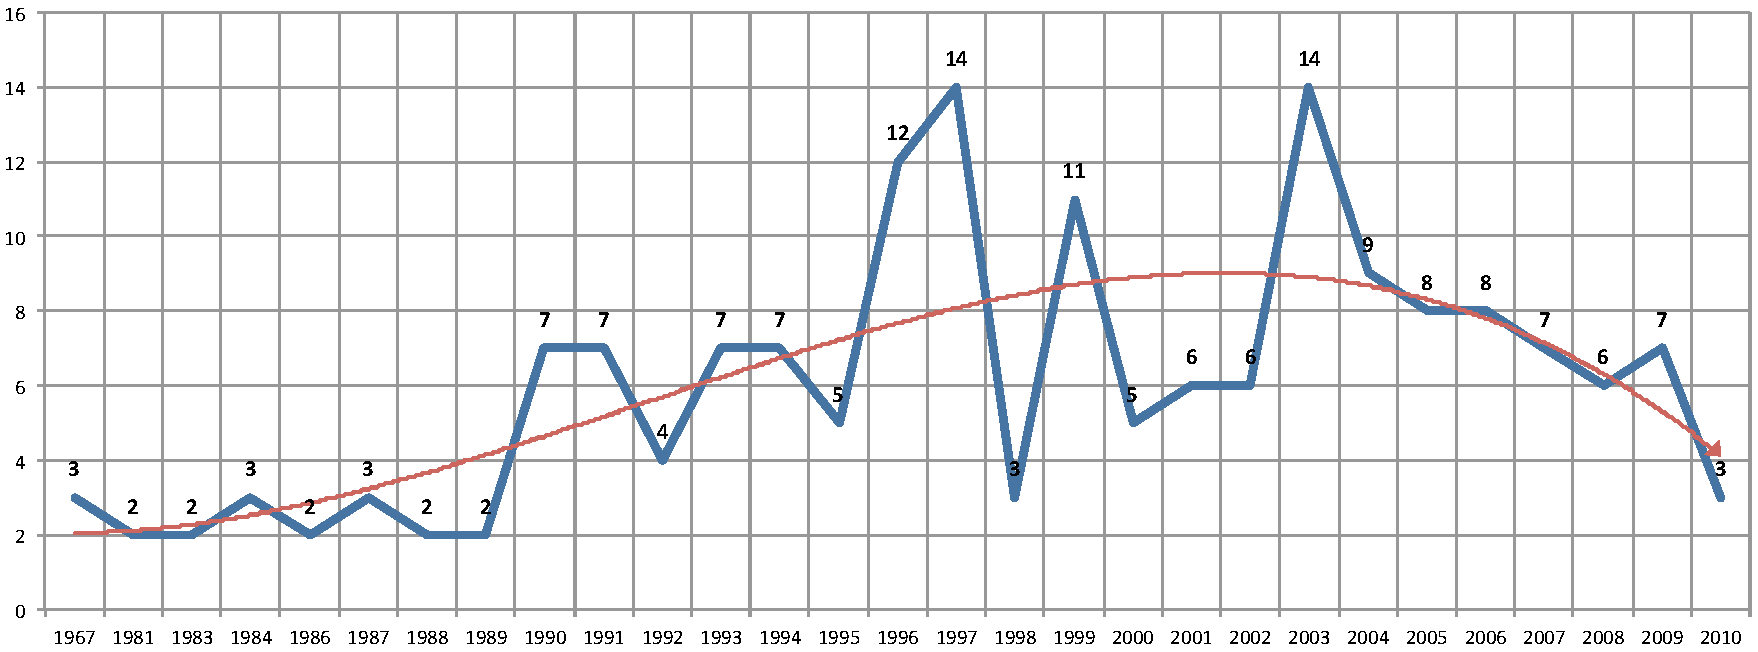
\includegraphics[scale=0.5]{img-grafico.pdf}
	\end{center}
	\caption{\label{fig_grafico}Gráfico produzido em Excel e salvo como PDF}
	\legend{Fonte: \textcite[24]{araujo2012}}
\end{figure}

% ---
\subsection{Figuras em \emph{minipages}}
% ---

\emph{Minipages} são usadas para inserir textos ou outros elementos em quadros com tamanhos e posições controladas. Veja o exemplo da \autoref{fig_minipage_imagem1} e da \autoref{fig_minipage_grafico2}.

\begin{figure}[htb]
 \label{teste}
 \centering
  \begin{minipage}{0.4\textwidth}
    \centering
    
\includegraphics[scale=0.9]{img-marca.pdf}
    \caption{Imagem 1 da minipage} \label{fig_minipage_imagem1}
    \legend{Fonte: Produzido pelos autores}
  \end{minipage}
  \hfill
  \begin{minipage}{0.4\textwidth}
    \centering
    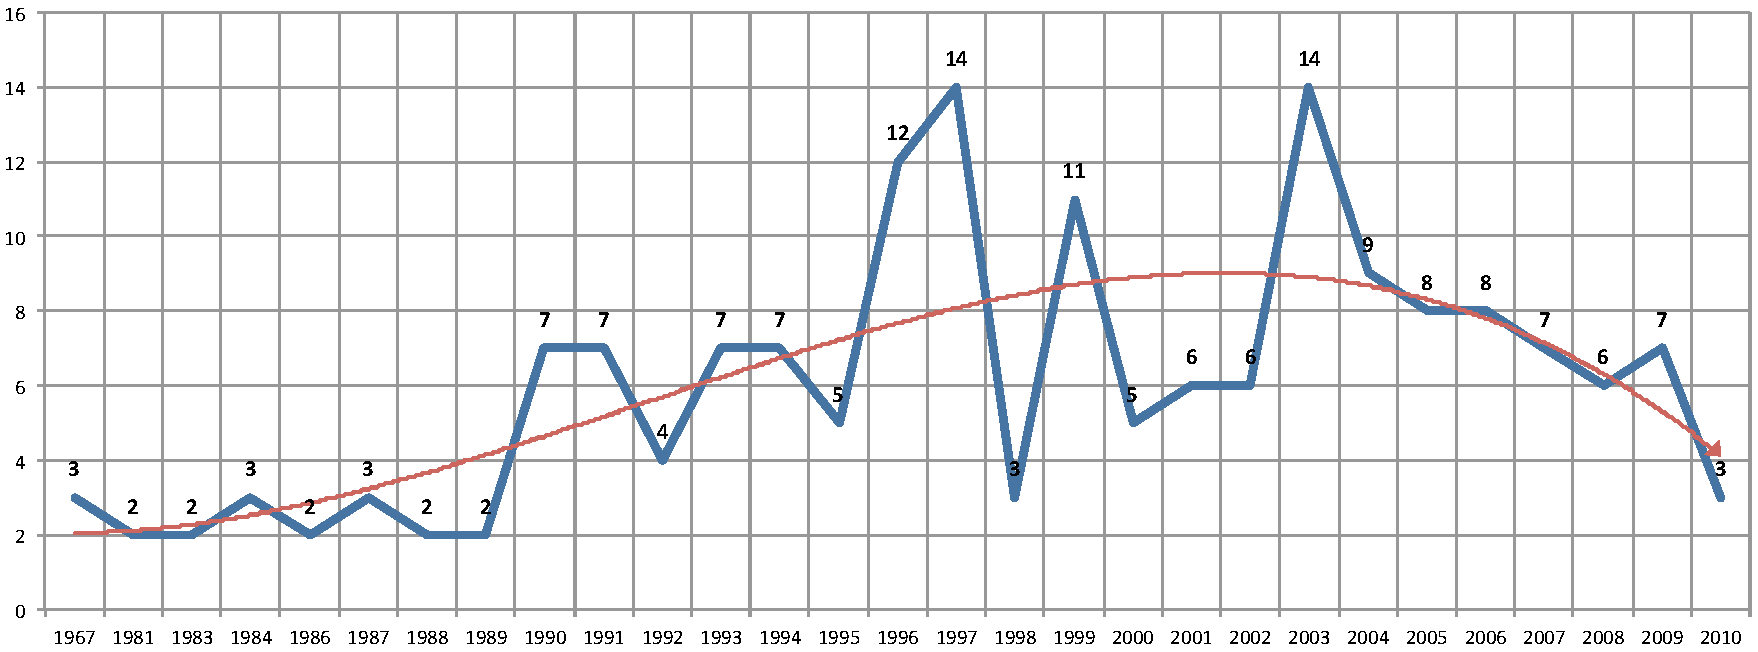
\includegraphics[scale=0.2]{img-grafico.pdf}
    \caption{Gráfico 2 da minipage} \label{fig_minipage_grafico2}
    \legend{Fonte: \textcite[24]{araujo2012}}
  \end{minipage}
\end{figure}

\subsection{Subfiguras}

\begin{figure}[H]
    \centering
	\begin{subfigure}[t]{0.4\columnwidth}
		
\includegraphics[scale=0.9]{img-marca.pdf}
		\caption{Primeira subfigura}
		\label{fig_subfigura_imagem1}
    \end{subfigure}%
    \hfill
    \begin{subfigure}[t]{0.4\columnwidth}
		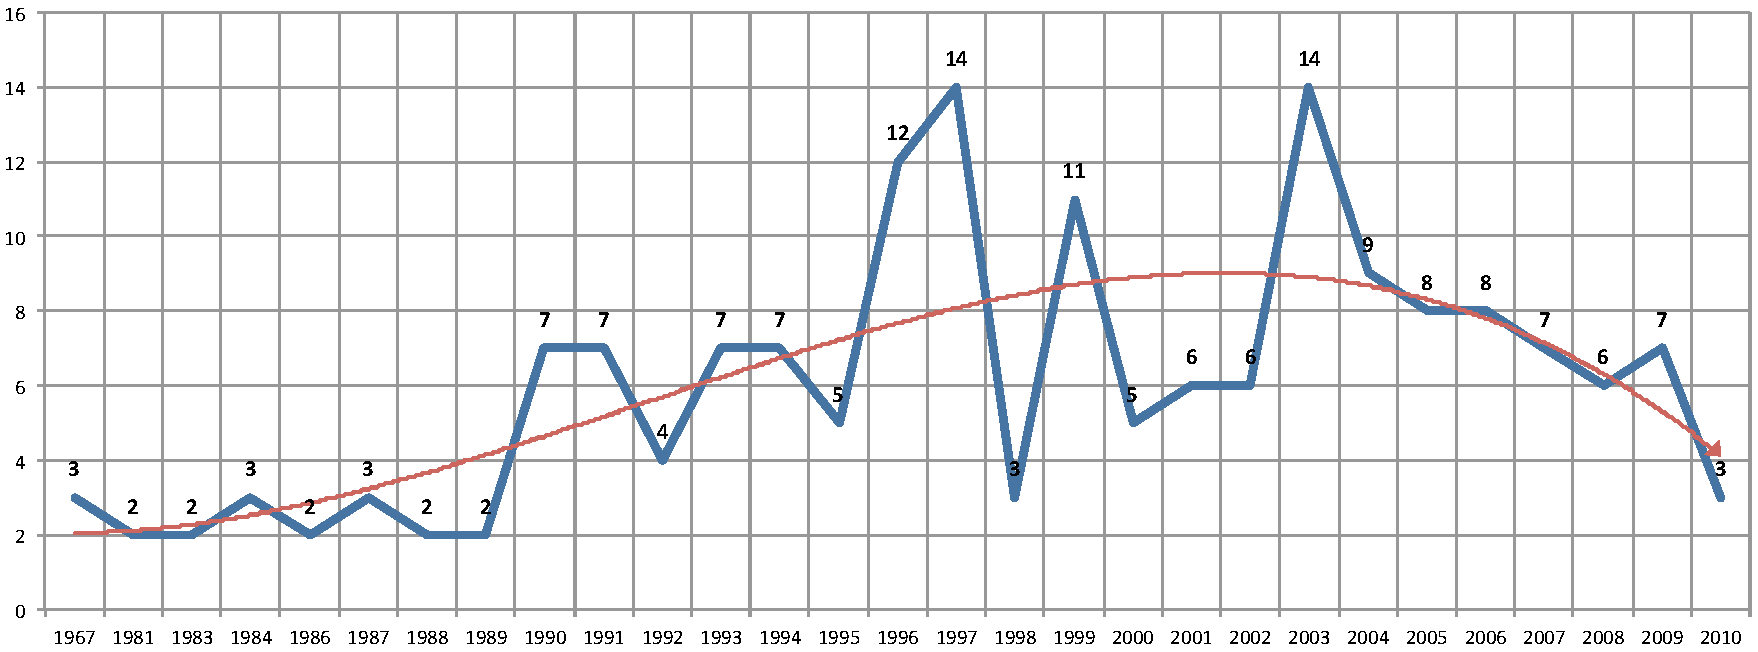
\includegraphics[scale=0.2]{img-grafico.pdf}
		\caption{Segunda subfigura}
		\label{fig_subfigura_grafico2}
    \end{subfigure}
    \caption{Figura com subfiguras}
    \label{fig:tau}
\end{figure}

Observe que, segundo a \textcite[seções 4.2.1.10 e 5.8]{NBR14724:2011}, as ilustrações devem sempre ter numeração contínua e única em todo o documento:

\begin{citacao}
Qualquer que seja o tipo de ilustração, sua identificação aparece na parte superior, precedida da palavra designativa (desenho, esquema, fluxograma, fotografia, gráfico, mapa, organograma, planta, quadro, retrato, figura, imagem, entre outros), seguida de seu número de ordem de ocorrência no texto, em algarismos arábicos, travessão e do respectivo título. Após a ilustração, na parte inferior, indicar a fonte consultada (elemento obrigatório, mesmo que seja produção do próprio autor), legenda, notas e outras informações necessárias à sua compreensão (se houver). A ilustração deve ser citada no texto e inserida o mais próximo possível do trecho a que se refere. \cite[seção 5.8]{NBR14724:2011}
\end{citacao}

% ---
\section{Expressões matemáticas}
\label{sec-mat}
% ---

Use o ambiente \texttt{equation} para escrever expressões matemáticas numeradas:

\begin{equation}
  \forall x \in X, \quad \exists \: y \leq \epsilon
\end{equation}

Escreva expressões matemáticas entre \$ e \$, como em $ \lim_{x \to \infty} \exp(-x) = 0 $, para que fiquem na mesma linha.

Também é possível usar colchetes para indicar o início de uma expressão matemática que não é numerada.

\[
\left|\sum_{i=1}^n a_ib_i\right|
\le
\left(\sum_{i=1}^n a_i^2\right)^{1/2}
\left(\sum_{i=1}^n b_i^2\right)^{1/2}
\]

Consulte mais informações sobre expressões matemáticas em \url{https://github.com/abntex/abntex2/wiki/Referencias}.

Muitos cientistas gostam de usar \LaTeX\ porque essa ferramenta possibilita escrever facilmente equações como a seguinte:

\begin{equation}
p+\frac{1}{2}{\rho}v^2+{\rho}gh = \text{constante}
 \label{eq:Bernoulli}
\end{equation}

\noindent onde $p$ é a pressão, $v$ é a velocidade e $h$ é a elevação, ou seja, a ``altura do tubo''. A \autoref{eq:Bernoulli} pode ser deduzida a partir do \textit{Teorema Trabalho-Energia}.

% Definição da nomenclatura que irá para a lista de símbolos
\nomenclature[B]{$p$}{Pressão}
\nomenclature[B]{$v$}{Velocidade}
\nomenclature[B]{$h$}{Elevação}

A seguir, são apresentados mais alguns exemplos de equações feitas com o \LaTeX.

\newcommand{\vt}[1]{\mathbf{#1}}

\begin{equation}\label{eq:R_f_usual}
\vt{R}_r(t) = \vt{R}_{\chi}(t) \triangleq 
\begin{bmatrix}
\cos \chi_0 (t) & -\sin \chi_0 (t) & 0
\\
\sin \chi_0 (t) & \cos \chi_0 (t) & 0
\\
0 & 0 & 1
\end{bmatrix},
\end{equation}

\begin{equation}
\vt{L}_{ij} = 
\begin{cases}
-a_{ij}, & \text{se } j \neq i \text{ e } j \in \mathcal{N}_i, \\
\sum_{k \in \mathcal{N}_i} a_{ik}, & \text{se } j = i,  \\
0, & \text{caso contrário},
\end{cases}
\end{equation}

\begin{align}
\tau_{li}^s(t) &= \ddot{p}^d_{li}(t) - k_{d} \dot{e}_{li}(t) - k_{p} e_{li}(t),
\\
\dot{\tau}_{li}^f(t) +  \xi_{i} \tau_{li}^f(t) &= u_{li}(t),\label{eq:filtro_i}
\\
u_{li}(t) &= - \textrm{sign}(s_{li}(t))\eta. \label{eq:u_xbi}
\end{align}

\begin{equation}\label{eq:point-mass-velocity}
\begin{split}
\dot{V}_i(t) &{}= \frac{T_i(t) - D_i(t)}{m_i} - g \sin \gamma_i(t) + b_{ti}(t), \\
\dot{\chi}_i(t) &{}= \frac{L_i(t) \sin \phi_i(t)}{m_i V_i(t) \cos \gamma_i(t)} + \frac{b_{\psi i}(t)}{V_i(t)\cos \gamma_i(t)},\\
\dot{\gamma}_i(t) &{}= \frac{L_i(t) \cos \phi_i(t)}{m_i V_i(t)} - \frac{g \cos \gamma_i(t)}{V_i(t)} + \frac{b_{\theta i}(t)}{V_i(t)},
\end{split}
\end{equation}

% ---
\section{Enumerações: alíneas e subalíneas}
% ---

Quando for necessário enumerar os diversos assuntos de uma seção que não possua título, esta deve ser
subdividida em alíneas \cite[seção 4.2]{NBR6024:2012}:

\begin{alineas}

  \item os diversos assuntos que não possuam título próprio, dentro de uma mesma   seção, devem ser subdivididos em alíneas; 
  \item o texto que antecede as alíneas termina em dois pontos;
  \item as alíneas devem ser indicadas alfabeticamente, em letra minúscula, seguida de parêntese. Utilizam-se letras dobradas, quando esgotadas as letras do alfabeto;
  \item as letras indicativas das alíneas devem apresentar recuo em relação à margem esquerda;
  \item o texto da alínea deve começar por letra minúscula e terminar em ponto-e-vírgula, exceto a última alínea que termina em ponto final;
  \item o texto da alínea deve terminar em dois pontos, se houver subalínea;
  \item a segunda e as seguintes linhas do texto da alínea começa sob a primeira letra do texto da própria alínea;
  \item subalíneas \cite[seção 4.3]{NBR6024:2012} devem ser conforme as alíneas a   seguir:

  \begin{alineas}
     \item as subalíneas devem começar por travessão seguido de espaço;
     \item as subalíneas devem apresentar recuo em relação à alínea;
     \item o texto da subalínea deve começar por letra minúscula e terminar em ponto-e-vírgula. A última subalínea deve terminar em ponto final, se não houver alínea subsequente;
     \item a segunda e as seguintes linhas do texto da subalínea começam sob a primeira letra do texto da própria subalínea.
  \end{alineas}
  
  \item no \abnTeX\ estão disponíveis os ambientes \texttt{incisos} e   \texttt{subalineas}, que em suma são o mesmo que se criar outro nível de \texttt{alineas}, como nos exemplos à seguir:
  
  \begin{incisos}
    \item \textit{Um novo inciso em itálico};
  \end{incisos}
  
  \item Alínea em \textbf{negrito}:
  
  \begin{subalineas}
    \item \textit{Uma subalínea em itálico};
    \item \underline{\textit{Uma subalínea em itálico e sublinhado}}; 
  \end{subalineas}
  
  \item Última alínea com \emph{ênfase}.
  
\end{alineas}

% ---
\section{Inclusão de outros arquivos}\label{sec-include}
% ---

É uma boa prática dividir o seu documento em diversos arquivos, e não apenas escrever tudo em um único. Esse recurso foi utilizado neste documento. Para incluir diferentes arquivos em um arquivo principal, de modo que cada arquivo incluído fique em uma página diferente, utilize o comando:

\begin{verbatim}
   \include{documento-a-ser-incluido}      % sem a extensão .tex
\end{verbatim}

Para incluir documentos sem quebra de páginas, utilize:

\begin{verbatim}
   \input{documento-a-ser-incluido}      % sem a extensão .tex
\end{verbatim}

% ---
\section{Remissões internas}
% ---

Ao nomear a \autoref{tab-nivinv} e a \autoref{fig:syscl}, apresentamos um exemplo de remissão interna, que também pode ser feita quando indicamos o \autoref{cap_exemplos}, que tem o nome \emph{\nameref{cap_exemplos}}. O número do capítulo indicado é \ref{cap_exemplos}, que se inicia à \autopageref{cap_exemplos}\footnote{O número da página de uma remissão pode ser obtida também assim:
\pageref{cap_exemplos}.}. Veja a \autoref{sec-divisoes} para outros exemplos de remissões internas entre seções, subseções e subsubseções.

O código usado para produzir o texto desta seção é:

\begin{verbatim}
Ao nomear a \autoref{tab-nivinv} e a \autoref{fig:syscl}, apresentamos um
exemplo de remissão interna, que também pode ser feita quando indicamos o
\autoref{cap_exemplos}, que tem o nome \emph{\nameref{cap_exemplos}}. O número
do capítulo indicado é \ref{cap_exemplos}, que se inicia à
\autopageref{cap_exemplos}\footnote{O número da página de uma remissão pode ser
obtida também assim:
\pageref{cap_exemplos}.}.
Veja a \autoref{sec-divisoes} para outros exemplos de remissões internas entre
seções, subseções e subsubseções.
\end{verbatim}

% ---
\section{Divisões do documento: seção}\label{sec-divisoes}
% ---

Esta seção testa o uso de divisões de documentos. Esta é a \autoref{sec-divisoes}. Veja a \autoref{sec-divisoes-subsection}.

\subsection{Divisões do documento: subseção}\label{sec-divisoes-subsection}

Isto é uma subseção. Veja a \autoref{sec-divisoes-subsubsection}, que é uma \texttt{subsubsection} do \LaTeX, mas é impressa chamada de ``subseção'' porque no Português não temos a palavra ``subsubseção''.

\subsubsection{Divisões do documento: subsubseção}
\label{sec-divisoes-subsubsection}

Isto é uma subsubseção.

\subsubsection{Divisões do documento: subsubseção}

Isto é outra subsubseção.

\subsection{Divisões do documento: subseção}\label{sec-exemplo-subsec}

Isto é uma subseção.

\subsubsection{Divisões do documento: subsubseção}

Isto é mais uma subsubseção da \autoref{sec-exemplo-subsec}.

\subsubsubsection{Esta é uma subseção de quinto nível}\label{sec-exemplo-subsubsubsection}

Esta é uma seção de quinto nível. Ela é produzida com o seguinte comando:

\begin{verbatim}
\subsubsubsection{Esta é uma subseção de quinto
nível}\label{sec-exemplo-subsubsubsection}
\end{verbatim}

\subsubsubsection{Esta é outra subseção de quinto nível}\label{sec-exemplo-subsubsubsection-outro}

Esta é outra seção de quinto nível.

\paragraph{Este é um parágrafo numerado}\label{sec-exemplo-paragrafo}

Este é um exemplo de parágrafo nomeado. Ele é produzida com o comando de parágrafo:

\begin{verbatim}
\paragraph{Este é um parágrafo nomeado}\label{sec-exemplo-paragrafo}
\end{verbatim}

A numeração entre parágrafos numeradaos e subsubsubseções são contínuas.

\paragraph{Esta é outro parágrafo numerado}\label{sec-exemplo-paragrafo-outro}

Esta é outro parágrafo nomeado.

% ---
\section{Este é um exemplo de nome de seção longo. Ele deve estar alinhado à esquerda e a segunda e demais linhas devem iniciar logo abaixo da primeira palavra da primeira linha}
% ---

Isso atende à norma \textcite[seções 5.2.2 a 5.2.4]{NBR14724:2011} e \textcite[seções 3.1 a 3.8]{NBR6024:2012}.

% ---
\section{Diferentes idiomas e hifenizações}
\label{sec-hifenizacao}
% ---

Para usar hifenizações de diferentes idiomas, inclua nas opções do documento o nome dos idiomas que o seu texto contém.

O idioma português-brasileiro (\texttt{brazil}) é incluído automaticamente pela classe \textsf{abntex2}. Porém, mesmo assim a opção \texttt{brazil} deve ser informada como a última opção da classe para que todos os pacotes reconheçam o idioma. Vale ressaltar que a última opção de idioma é a utilizada por padrão no documento.

A lista completa de idiomas suportados, bem como outras opções de hifenização, estão disponíveis em \textcite[5-6]{babel}.

Exemplo de hifenização em inglês\footnote{Extraído de: \url{http://en.wikibooks.org/wiki/LaTeX/Internationalization}}:

\begin{otherlanguage*}{english}
\textit{Text in English language. This environment switches all language-related definitions, like the language specific names for figures, tables etc. to the other language. The starred version of this environment typesets the main text according to the rules of the other language, but keeps the language specific string for ancillary things like figures, in the main language of the document. The environment hyphenrules switches only the hyphenation patterns used; it can also be used to disallow hyphenation by using the language name `nohyphenation'.}
\end{otherlanguage*}

O idioma geral do texto por ser alterado como no exemplo seguinte:

\begin{verbatim}
  \selectlanguage{english}
\end{verbatim}

Isso altera automaticamente a hifenização e todos os nomes constantes de referências do documento para o idioma inglês. Consulte o manual da classe \cite{abntex2classe} para obter orientações adicionais sobre internacionalização de documentos produzidos com \abnTeX.

A \autoref{sec-citacao} descreve o ambiente \texttt{citacao} que pode receber como parâmetro um idioma a ser usado na citação.

% ---
\section{Consulte o manual da classe \textsf{abntex2}}
% ---

Consulte o manual da classe \textsf{abntex2} \cite{abntex2classe} para uma referência completa das macros e ambientes disponíveis. 

Além disso, o manual possui informações adicionais sobre as normas ABNT observadas pelo \abnTeX\ e considerações sobre eventuais requisitos específicos não atendidos, como o caso da \textcite[seção 5.2.2]{NBR14724:2011}, que especifica o espaçamento entre os capítulos e o início do texto, regra propositalmente não atendida pelo presente modelo.

% ---
\section{Referências bibliográficas}
% ---

Para referências bibliográficas que seguem as normas da ABNT são utilizados os pacotes \textsf{biblatex} e \textsf{biblatex-abnt}. Consulte os manuais \textcite{biblatex} e \textcite{biblatexabnt} para obter informações sobre como utilizar as referências bibliográficas.

Embora as normas da ABNT permitam citações utilizando o formato numérico, é recomendado o uso do sistema autor-ano em trabalhos acadêmicos. A razão é que a leitura por parte do avaliador fica mais simples. Basta ver o nome e o ano para se lembrar rapidamente da referência, sem precisar recorrer frequentemente à lista de referências, que fica no final do texto, tornando a leitura mais agradável.

No formato autor-data, considere chamar as referências usando o comando \verb|\textcite| com maior frequência que o comando \verb|\cite|. Desse modo, a citação fica melhor incorporada ao texto, outra vantagem do formato autor-data

% ---
\section{Listas}
% ---

As listas de ilustrações (figuras) e de tabelas utilizadas ao longo do trabalho são geradas automaticamente e incluídas entre o \emph{Abstract} e o Sumário.

Para definir um elemento que deverá aparecer na lista de abreviatura e siglas, próximo do texto onde a sigla ou abreviatura aparece, utilize o comando \verb|\nomenclature|. Por exemplo, para definir as siglas que aparecem no primeiro parágrafo do \autoref{cap_intr}, foram utilizados os seguintes comandos:

\begin{verbatim}
\nomenclature[A]{ABNT}{Associação Brasileira de Normas Técnicas}
\nomenclature[A]{UnB}{Universidade de Brasília}
\end{verbatim}

Para definir um elemento da lista de símbolos, próximo da equação onde o símbolo aparece, utilize também o comando \verb|\nomenclature|. Por exemplo, para definir os símbolos das equações da \autoref{sec-mat}, foram utilizados os comandos:

\begin{verbatim}
\nomenclature[B]{$p$}{Pressão}
\nomenclature[B]{$v$}{Velocidade}
\nomenclature[B]{$h$}{Elevação}
\end{verbatim}

Note que o \verb|[A]| de \verb|\nomenclature[A]| indica que se trata de uma abreviatura ou sigla. Já o \verb|[B]| em \verb|\nomenclature[B]| indica que se trata de símbolo. Daí cada elemento a ser listado vai para a lista a qual pertencem.

% ---
\section{Ficha catalográfica com código Cutter-Sanborn}
% ---
A Tabela Cutter-Sanborn é uma codificação elaborada por Charles Ammi Cutter e, posteriormente, expandida por Kate F. Sanborn. Na Tabela Cutter-Sanborn, é possível consultar qual sequência numérica representa a sequência do sobrenome do autor.

Em vários sites da internet\footnote{\url{https://www.tabelacutter.com/}}\footnote{\url{https://cuttersonline.com.br/registrador-gratuito}} há ferramentas online para obtenção do código. Se o nome do primeiro autor do trabalho for, digamos, Carlos Lisboa, a entrada da ferramenta online deverá ser: \textbf{Lisboa, Carlos}. Nenhuma outra informação é necessária para gerar o código que, no caso desse autor, é \textbf{769}. Considere apenas esses três números. Eventuais letras devem ser ignoradas. No arquivo \verb|*.tex| principal do relatório, na linha que tem o comando \verb|\numerocutter| troque por

\begin{verbatim}
\numerocutter{769}
\end{verbatim}

Esse número aparecerá na ficha catalográfica gerada. Automaticamente será adicionado na frente do número, a letra \textbf{L} maiúscula, que é a primeira letra do sobrenome \textbf{Lisboa}. Será também adicionado, ao final do número, a letra \textbf{m} minúscula, correspondente à primeira letra do título do trabalho (o título desse relatório de exemplo é ``Modelo de Trabalho Acadêmico com UnB\TeX''). Se seu nome for, por exemplo, Carlos da Silva, utilize como entrada da ferramenta que gera o código: \textbf{Silva, Carlos da}.

A ficha catalográfica é um elemento pré-textual obrigatório para todos os trabalhos acadêmicos (teses, dissertações e trabalhos de conclusão de curso: graduação e especialização).
% ---

% ---
% Capítulo com a proposta desenvolvida
% ---
% ----------------------------------------------------------
\chapter{Figuras e gráficos}
% ----------------------------------------------------------

\section{Introdução}

Sugiro que você guarde todas as figuras na pasta ``figuras'' para que seu projeto fique mais organizado. A figura \ref{fig:logolatex} mostra como é fácil inserir uma figura com legenda e referência à fonte.

\begin{figure}[htb]
	\centering
	\begin{minipage}{0.6\linewidth}
		\centering
		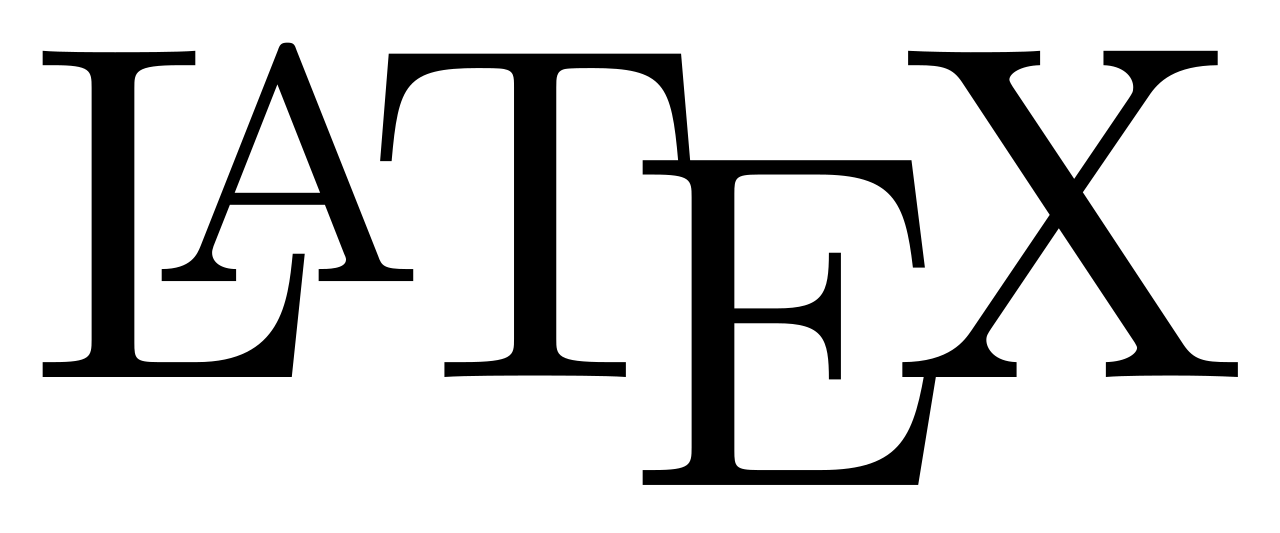
\includegraphics[width=\linewidth]{1280px-LaTeX-logo.png}
		\caption{Logo \LaTeX.} \label{fig:logolatex}
		\source{Wikimedia Commons \cite{wikimedia-latex}.}
	\end{minipage}
\end{figure}

Além de figuras, é possível inserir caixas de texto de diversos tipos, como axiomas, teoremas etc.

Existem pacotes que permitem criar figuras e gráficos no próprio código \LaTeX. Por exemplo, temos

\begin{itemize}
    \item PGFPlots \url{http://pgfplots.sourceforge.net/}
    \item TikZ \url{http://www.texample.net/tikz/examples/all/}
    \item Metapost \url{http://tex.loria.fr/prod-graph/zoonekynd/metapost/metapost.html}
    \item PSTricks \url{https://tug.org/PSTricks/main.cgi?file=examples}
\end{itemize}

\section{Exercício}

\begin{exercise}
    Explique como Isaac Newton usaria cada um dos pacotes seguintes, se vivesse no tempo presente:
    \begin{enumerate}[label=(\Alph*)]
        \item Metapost
        \item TikZ
        \item PGFPlots
        \item PSTricks
    \end{enumerate}
\end{exercise}

%\begin{solution}
%    \begin{enumerate}[label=(\Alph*)]
%        \item Para fazer figuras 3D.
%        \item Para fazer diagramas.
%        \item Para traçar gráficos.
%        \item Para fazer de um tudo.
%    \end{enumerate}
%\end{solution}

\section{Algoritmo}

\begin{algorithm} [h]
\caption{NN-based MPC pseudocode for consensus control}
\label{alg:NNMPC}
\begin{algorithmic}[1]

%\Procedure{Roy}{$a,b$}       \Comment{This is a test}
    \State System Initialization at $x(0), \theta(0)$
    \State $J = V(e(0),\theta(0))$
    \State $K^{ab}_0 = 0$ $\forall (a,b)$
    \State $dataset \gets [K_0,J]$
    \For{$k = 1:k_{max}$} \Comment{Simulation loop}
        \State $(W,Y) \gets train(dataset)$
        \State $\tilde{J} = Y\sigma(Wz)$ $\forall K^{ab}_k\pm \delta_K
        $
        \State $K_k^{\ast} = arg \min_{K_k}(\tilde{J})$
        \State $u(k) =  \left( L(\theta(k)) \otimes K_k^{\ast} \right) x(k)$
        \State $\hat{x}(k) = x(k)$; $\hat{\theta}(k) = \theta(k)$
        \For{$t = k+1:k+h+1$} \Comment{Prediction loop}
            %\For{$s = 1:S$} \Comment{Markov loop}
                \State $\hat{\theta}(t) = randMarkov(\hat{\theta}(t-1),\Pi)$
                \State $p = \hat{\theta}(t)$
                \State $\hat{u}(t) = \left( L(p) \otimes K_k^{\ast} \right) \hat{x}(t)$
                \State $\hat{x}(t+1) = F_p(\hat{x}(t))$
                \State $x_0(t) = mean(\hat{x}(t))$
                \State $\hat{e}(t) = F_p(\hat{x}(t)) - \boldsymbol{1_N} f_{p0}(x(t)) $
                \State $\hat{V}_t = \hat{e}^T(t)P_{p}\hat{e}(t)$
                \EndFor
                %\State $r(t) = r(t-k)\Pi^{k}$
                %\State $\bar{V}_t = \sum_{s=1}^S r_s(t) V_t^s$
                %\EndFor
        \State $\hat{J} = \sum_{t = k+1}^{k+h+1} \hat{V}_t$
        \State $dataset \gets [K^{\ast}_k,\hat{J}]$
        \State $x(k+1) = F_p(x(k))$
    \EndFor
    
%\EndProcedure

\end{algorithmic}
\end{algorithm}

\section{Programa}

\begin{lstlisting}
/**
* MSO: ativa o servo cujo eixo eh descrito
* por drive_axis; informacoes de controle
* sao gravadas em MSO_1
*/
  MSO(drive_axis,MSO_1);
/* Atribui o valor 0.0 ao primeiro elemento do array speed */
  speed[0] := 0.0; 
/* Atribui 1 para dataInitialized */
  dataInitialized := 1;
\end{lstlisting}

Para mais exemplos de programas, veja o \autoref{apd:cdg}
% ---

% ---
% Capítulo de resultados
% ---
% ----------------------------------------------------------
\chapter{Ambientes}
% ----------------------------------------------------------

Este modelo disponibiliza alguns ``ambientes'', ou seja, caixas de texto com formatação especial para certos tipos de elementos que são automaticamente numerados (e.g. teorema 1.1, teorema 1.2 etc.). Esses ambientes foram adaptados para o UnB\TeX\ a partir soluções utilizadas por \textcite{Castro2019}.

\section{Exemplos de ambientes disponíveis}

%\begin{axiom}
%    \LaTeX produz equações mais bonitas que qualquer editor WYSIWYG.
%\end{axiom}

\begin{definition}
O WYSIWYG (ou ``What You See Is What You Get - O que você vê é o formato final'') é um tipo de editor HTML que permite editar sua página da Web em uma visualização simplificada e sem código de aparência semelhante à do layout da página real.
\end{definition}

\begin{proposition}
    \LaTeX\ produz equações mais bonitas que qualquer editor WYSIWYG.
\end{proposition}

\begin{lemma}
    Teste
\end{lemma}

\begin{remark}
    \LaTeX\ produz equações mais bonitas que qualquer editor WYSIWYG.
\end{remark}

\begin{theorem}[Teorema LaTeX-WYSIWYG]\label{thm:WYSIWYG}
    Todo físico prefere usar código \LaTeX\ puro que qualquer editor WYSIWYG.
\end{theorem}

\begin{corollary}
    Teste
\end{corollary}

\begin{proof}
    Físicos gostam de equações bonitas. Editores What-You-See-Is-What-You-Get não são apropriados para fazer equações bonitas.\footnote{É certo que há editores WYSIWYG baseados em \LaTeX, mas eles não nos dão o mesmo nível de controle.} Logo, se algum físico preferisse usar um editor WYSIWYG no lugar de \LaTeX, não seria muito inteligente. Como todo físico é inteligente, o teorema está demonstrado \textit{ad absurdum}.
\end{proof}

\begin{example}
    Einstein usaria um editor WYSIWYG ou \LaTeX? \\
    Einstein era físico. Portanto, usando o teorema LaTeX-WYSIWYG, concluímos que ele usaria \LaTeX.
\end{example}

O \autoref{thm:WYSIWYG} é um exemplo de teorema.

%\begin{exercise}
%    Einstein usaria um editor WYSIWYG ou \LaTeX?
%\end{exercise}

%\begin{solution}
%    Einstein era físico. Portanto, usando o teorema LaTeX-WYSIWYG, concluímos que ele usaria \LaTeX.
%\end{solution}

\begin{exercise}
    Marie Curie usaria um editor WYSIWYG ou \LaTeX?
\end{exercise}

\begin{exercise}
    Deixamos esta sem resposta para o estudante se esforçar mais.
\end{exercise}
% ---

% ---
% Capítulo de conclusões
% ---
% ----------------------------------------------------------
\chapter{Conclusões}
% ----------------------------------------------------------

Você deve começar a editar o seu TG/Dissertação/Tese agora mesmo!
% ---

% ------------------------------------------------------------------------
% ELEMENTOS PÓS-TEXTUAIS
% ------------------------------------------------------------------------
\postextual
% ------------------------------------------------------------------------

% ---
% Referências bibliográficas
% ---

\defbibheading{bibliography}[\bibname]{\chapter*{#1}}
\cleardoublepage
\phantomsection
\tocprintchapternonum
\addcontentsline{toc}{chapter}{\texorpdfstring{\MakeTextUppercase{\bibname}}{\bibname}}
\printbibliography
\markboth{}{}
% ---

%\defbibheading{bibliography}[\refname]{\section*{#1}\sectionmark{\refname}}

% ---
% Apêndices
% ---

\begin{apendicesenv}

% Imprime uma página indicando o início dos apêndices
\partapendices

% ----------------------------------------------------------
\chapter{Citações}
% ----------------------------------------------------------

Este modelo usa Bib\LaTeX\ para configurar as referências. Os arquivo referencias.bib e references.bib contêm várias entradas de bibliografia como modelos \cite{article,book,booklet,inbook}. Esses modelos podem ser utilizados para incluir outras entradas e citá-las por meio do seguinte comando:
\begin{verbatim}
\cite{nome_da_entrada}
\end{verbatim}

Por exemplo , a entrada
%\verbatimfont{\small}
\begin{verbatim}
@article{greenwade93,
    author  = "George D. Greenwade",
    title   = "The {C}omprehensive {T}ex {A}rchive {N}etwork ({CTAN})",
    year    = "1993",
    journal = "TUGBoat",
    volume  = "14",
    number  = "3",
    pages   = "342--351"
}
\end{verbatim}
%\verbatimfont{\normalfont}
pode ser citada no texto com
\begin{verbatim}
\cite{greenwade93}
\end{verbatim}
e a citação apareceria assim: \cite{greenwade93}.

Para fazer uma citação direta no formato ABNT, criamos o ambiente \verb|citacao|, que é uma simples generalização do ambiente \verb|quotation| (habilitado por padrão) com um campo específico de autor. Veja o exemplo a seguir:
\begin{verbatim}
\begin{citacao}{Carl Sagan}
    Alegações extraordinárias exigem evidências extraordinárias.
\end{citacao}
\end{verbatim}
Esse código gera uma citação assim:
\begin{citacao}{Carl Sagan}
    Alegações extraordinárias exigem evidências extraordinárias.
\end{citacao}
O comando \verb|\cite{...}| pode ser usado como indicação do autor:
\begin{verbatim}
\begin{citacao}{\cite{greenwade93}}
TEX is a typesetting program designed for high-quality composition of material
that contains a lot of mathematical and technical expressions. It has been 
adopted by many authors and publishers who generate technical books and papers. 
It was created by Professor Donald E. Knuth of Stanford University, originally 
for preparation of his book series ``The Art of Computer Programming''. TEX 
has been made freely available by Knuth.
\end{citacao}
\end{verbatim}
Naturalmente, a referência \verb|grennwade93| deve estar definida no arquivo BibTeX (aqui, \verb|references.bib|). Confira o resultado:
\begin{citacao}{\cite{greenwade93}}
TEX is a typesetting program designed for high-quality composition of material that contains a lot of mathematical and technical expressions. It has been adopted by many authors and publishers who generate technical books and papers. It was created by Professor Donald E. Knuth of Stanford University, originally for preparation of his book series ``The Art of Computer Programming''. TEX has been made freely available by Knuth.
\end{citacao}

% ----------------------------------------------------------
\chapter{Códigos de programação}\label{apd:cdg}
% ----------------------------------------------------------

\section{Projeto do Controlador com Realimentação de Estados}
\lstinputlisting[language=Matlab,caption=Código de Matlab]{unbtex-example/codigos/controle.m}

\section{Exemplo de teste em Malha Fechada com Rampa}
\lstinputlisting[language=Python,caption=Código de Python]{unbtex-example/codigos/controleSmithPredictor.py}

\section{Redução modal}
\lstinputlisting[language=Julia,caption=Código de Julia]{unbtex-example/codigos/ModalReduction.jl}

\end{apendicesenv}
% ---

% ---
% Anexos
% ---

\begin{anexosenv}

% Imprime uma página indicando o início dos anexos
\partanexos

% ----------------------------------------------------------
\chapter{Figuras de exemplo}
% ----------------------------------------------------------

% Fonte: https://tex.stackexchange.com/a/231741/91816 (Gonzalo Medina)

\noindent\includegraphics[width=3cm]{example-image-a}\qquad
\includegraphics[width=3cm]{example-image-golden}\qquad
\includegraphics[width=3cm]{example-grid-100x100pt}

\noindent\includegraphics[height=5cm]{example-image-b} 

\noindent\includegraphics[scale=0.5]{example-image-c} 

\noindent\includegraphics[width=3cm]{example-image} 

% ----------------------------------------------------------
\chapter{Logo LaTeX}
% ----------------------------------------------------------

\vfill

\begin{center}
{\fontsize{50pt}{800pt}\selectfont \LaTeX}\
\end{center}

\vfill

\begin{center}
{\color{azulunb}\fontsize{50pt}{800pt}\selectfont \LaTeX}\
\end{center}

\vfill

\begin{center}
{\color{verdeunb}\fontsize{50pt}{800pt}\selectfont \LaTeX}\
\end{center}

\vfill

\end{anexosenv}

\end{document}